\documentclass[10pt,journal,compsoc]{IEEEtran}
\usepackage{cite}
\usepackage{amsmath,amssymb,amsfonts}
\usepackage{algorithmic}
\usepackage{algorithm}
\usepackage{graphicx}
\usepackage{textcomp}
\usepackage{xcolor}
\usepackage{booktabs}
\usepackage{hyperref}
\usepackage{multirow}
\usepackage{array}
\usepackage{url}

\hypersetup{colorlinks=true,linkcolor=blue,citecolor=blue,urlcolor=blue}

\begin{document}

\title{SEAL: Evaluating Orthogonal Subspace and Sparse Low-Rank Adaptation Under Autonomous Self-Directed Curricula in Continual Learning}

\author{Altamash~Shaikh,~\IEEEmembership{B.Tech AI \& ML, TCET Mumbai}
\IEEEcompsocitemizethanks{
  \IEEEcompsocthanksitem Submitted for Research Methodology Internal Examination, 2026.
  \IEEEcompsocthanksitem Code: \url{https://github.com/shaikhaltamash69/SEAL-Orthogonal-Continual-Learning}
}}

\IEEEtitleabstractindextext{
\begin{abstract}
Parameter-Efficient Fine-Tuning (PEFT) methods, particularly Subspace-Orthogonal Low-Rank Adaptation (O-LoRA) and Reduced Interference LoRA (LoRI), mitigate catastrophic forgetting in Large Language Models (LLMs) by restricting weight updates to orthogonal or sparsified parameter subspaces. However, all existing evaluations strictly assume static, human-curated task curricula---a condition fundamentally violated in autonomous self-editing architectures (e.g., SEAL) where the model autonomously synthesizes training data and directs its own edit sequence. This paper presents SEAL (Self-Edit Aware Learning), the first comprehensive empirical investigation of PEFT continual learning under model-directed, self-generated curricula across a complete $2 \times 2$ factorial matrix (O-LoRA vs. LoRI $\times$ Planned vs. Self-Gen). Evaluating across 19 sequential post-2024 verified factual updates over 3 random seeds (15 full runs, 285 sequential edit steps) using Qwen2.5-1.5B-Instruct on an NVIDIA RTX 4500 Ada GPU, our findings demonstrate: (1) Unconstrained self-editing suffers catastrophic forgetting ($0.0263 \pm 0.0215$ mean retention accuracy); (2) O-LoRA mitigates forgetting under self-directed curricula ($0.1228 \pm 0.0248$, a $+366.7\%$ improvement over baseline), but exhibits an empirical Curriculum Transfer Gap (CTG) of $+0.0088$ compared to human-planned ordering ($0.1316 \pm 0.0000$); (3) Sparse random projection methods (LoRI) eliminate curriculum vulnerability entirely, achieving superior retention under autonomous curricula ($0.1404 \pm 0.0124$, a $+433.3\%$ relative improvement over baseline, negative CTG of $-0.0088$). Qualitative trace inspection reveals that LLM self-selection exhibits semantic topic clustering, inducing localized parameter-space crowding that soft Frobenius orthogonality penalties fail to resolve. Finally, we formulate a multi-layered cryptographic watermarking protocol to safeguard continual learning intellectual property against unauthorized distillation and adapter theft.
\end{abstract}
\begin{IEEEkeywords}
Continual Learning, Low-Rank Adaptation, Catastrophic Forgetting, O-LoRA, LoRI,
Autonomous Self-Editing, SEAL, Curriculum Learning, Subspace Orthogonality.
\end{IEEEkeywords}}

\maketitle
\IEEEdisplaynontitleabstractindextext
\IEEEpeerreviewmaketitle

\section{Introduction}
\IEEEPARstart{L}{arge} Language Models (LLMs) are increasingly deployed in dynamic real-world environments demanding continuous knowledge acquisition. A deployed model must integrate newly verified facts without overwriting previously established knowledge. This challenge, termed catastrophic forgetting [1], remains one of the fundamental unsolved problems in machine learning.

Continual Learning (CL) research has produced a rich taxonomy of mitigation strategies: experience replay [2], and parameter-efficient subspace methods [3]. Among the latter, Low-Rank Adaptation (LoRA) [4] has emerged as the dominant paradigm. LoRA injects trainable rank-$r$ decomposition matrices into frozen transformer layers. Building on this, O-LoRA [5] enforces explicit orthogonality penalties between successive adapters, and LoRI [6] freezes the projection matrix using sparse random Gaussian projections.

A critical gap exists across all prior work: every PEFT continual learning algorithm is evaluated exclusively on human-curated task curricula. The emergence of autonomous self-editing architectures (SEAL [7]) violates this assumption entirely --- in SEAL systems, the LLM generates its own training data and self-selects the next edit target. This introduces the Curriculum Transfer Gap (CTG): the performance discrepancy between PEFT methods under human-planned versus model-generated curricula.

Contributions: (1) We formally define the CTG as the performance difference between PEFT under human-planned and self-generated curricula. (2) We present the first controlled empirical study of a complete $2 \times 2$ factorial PEFT design (O-LoRA vs. LoRI $\times$ Planned vs. Self-Gen) under autonomous self-editing on 19 post-2024 factual updates across 3 random seeds (15 full runs). (3) We demonstrate that LoRI eliminates the CTG entirely and achieves highest overall retention ($14.04\%$). (4) We document semantic topic clustering as a novel mechanism causing subspace crowding in self-directed learning.

\section{Related Work}

\subsection{Catastrophic Forgetting and Continual Learning}
Catastrophic forgetting [1] describes abrupt performance loss on prior tasks during sequential training. Mitigation strategies include experience replay [2], DualPrompt [3], EWC, and Progressive Neural Networks. LoRA [4] demonstrated that LLM weight updates are approximately low-rank, and QLoRA [8] extended this to quantized models enabling large-scale fine-tuning on consumer hardware.

\subsection{Orthogonal Subspace Methods}
O-LoRA [5] is the first to combine orthogonality constraints with LoRA for CL, enforcing adapter orthogonality via Frobenius-norm penalty. OPLoRA [9] extends this with hard projection via QR decomposition, providing stronger theoretical guarantees. The Lie Group approach [10] reformulates LoRA within the geometric structure of orthogonal matrices for improved numerical stability.

\subsection{Sparse Projection and Task-Free Methods}
LoRI [6] prevents interference by freezing A with sparse Gaussian random projections and applying top-k gradient masking to B. Online-LoRA [11] addresses task-free CL via dynamic rank expansion based on singular value monitoring, but assumes external data streams.

\subsection{Autonomous Self-Editing}
SEAL [7] introduced self-editing LLMs that update their own weights from self-generated data. Unlike prior CL work, SEAL creates a model-controlled curriculum, motivating our investigation of how PEFT methods behave under this fundamentally different learning paradigm.

\section{Literature Survey}

A systematic review of the five primary references reveals a universal assumption: curriculum order is always controlled by an external agent. Table I compares methods across dimensions relevant to autonomous self-editing.

TABLE I: Systematic Comparison of PEFT Continual Learning Methods
| Paper         | Venue         | Orthog.      | Sparse | Task-Free | Self-Edit | Key Limitation                        |
|---------------|---------------|--------------|--------|-----------|-----------|---------------------------------------|
| O-LoRA [5]    | EMNLP 2023    | Yes (soft)   | No     | No        | No        | Soft penalty insufficient under clustering |
| LoRI [6]      | arXiv 2025    | No           | Yes    | No        | No        | Only human-curated sequences tested   |
| OPLoRA [9]    | arXiv 2025    | Yes (hard)   | No     | No        | No        | High projection overhead              |
| Lie Grp [10]  | arXiv 2025    | Yes (manif.) | No     | No        | No        | Not tested on factual CL             |
| Online-LoRA[11]| WACV 2025    | No           | No     | Yes       | No        | Assumes external data stream          |
| SEAL (Ours)   | This Work     | Yes          | Yes    | No        | Yes       | First self-generated curriculum study |

None of the surveyed works investigates model-directed curriculum selection, confirming the novelty of our contribution.

\section{Methodology and System Architecture}

\begin{figure*}[t]
\centering
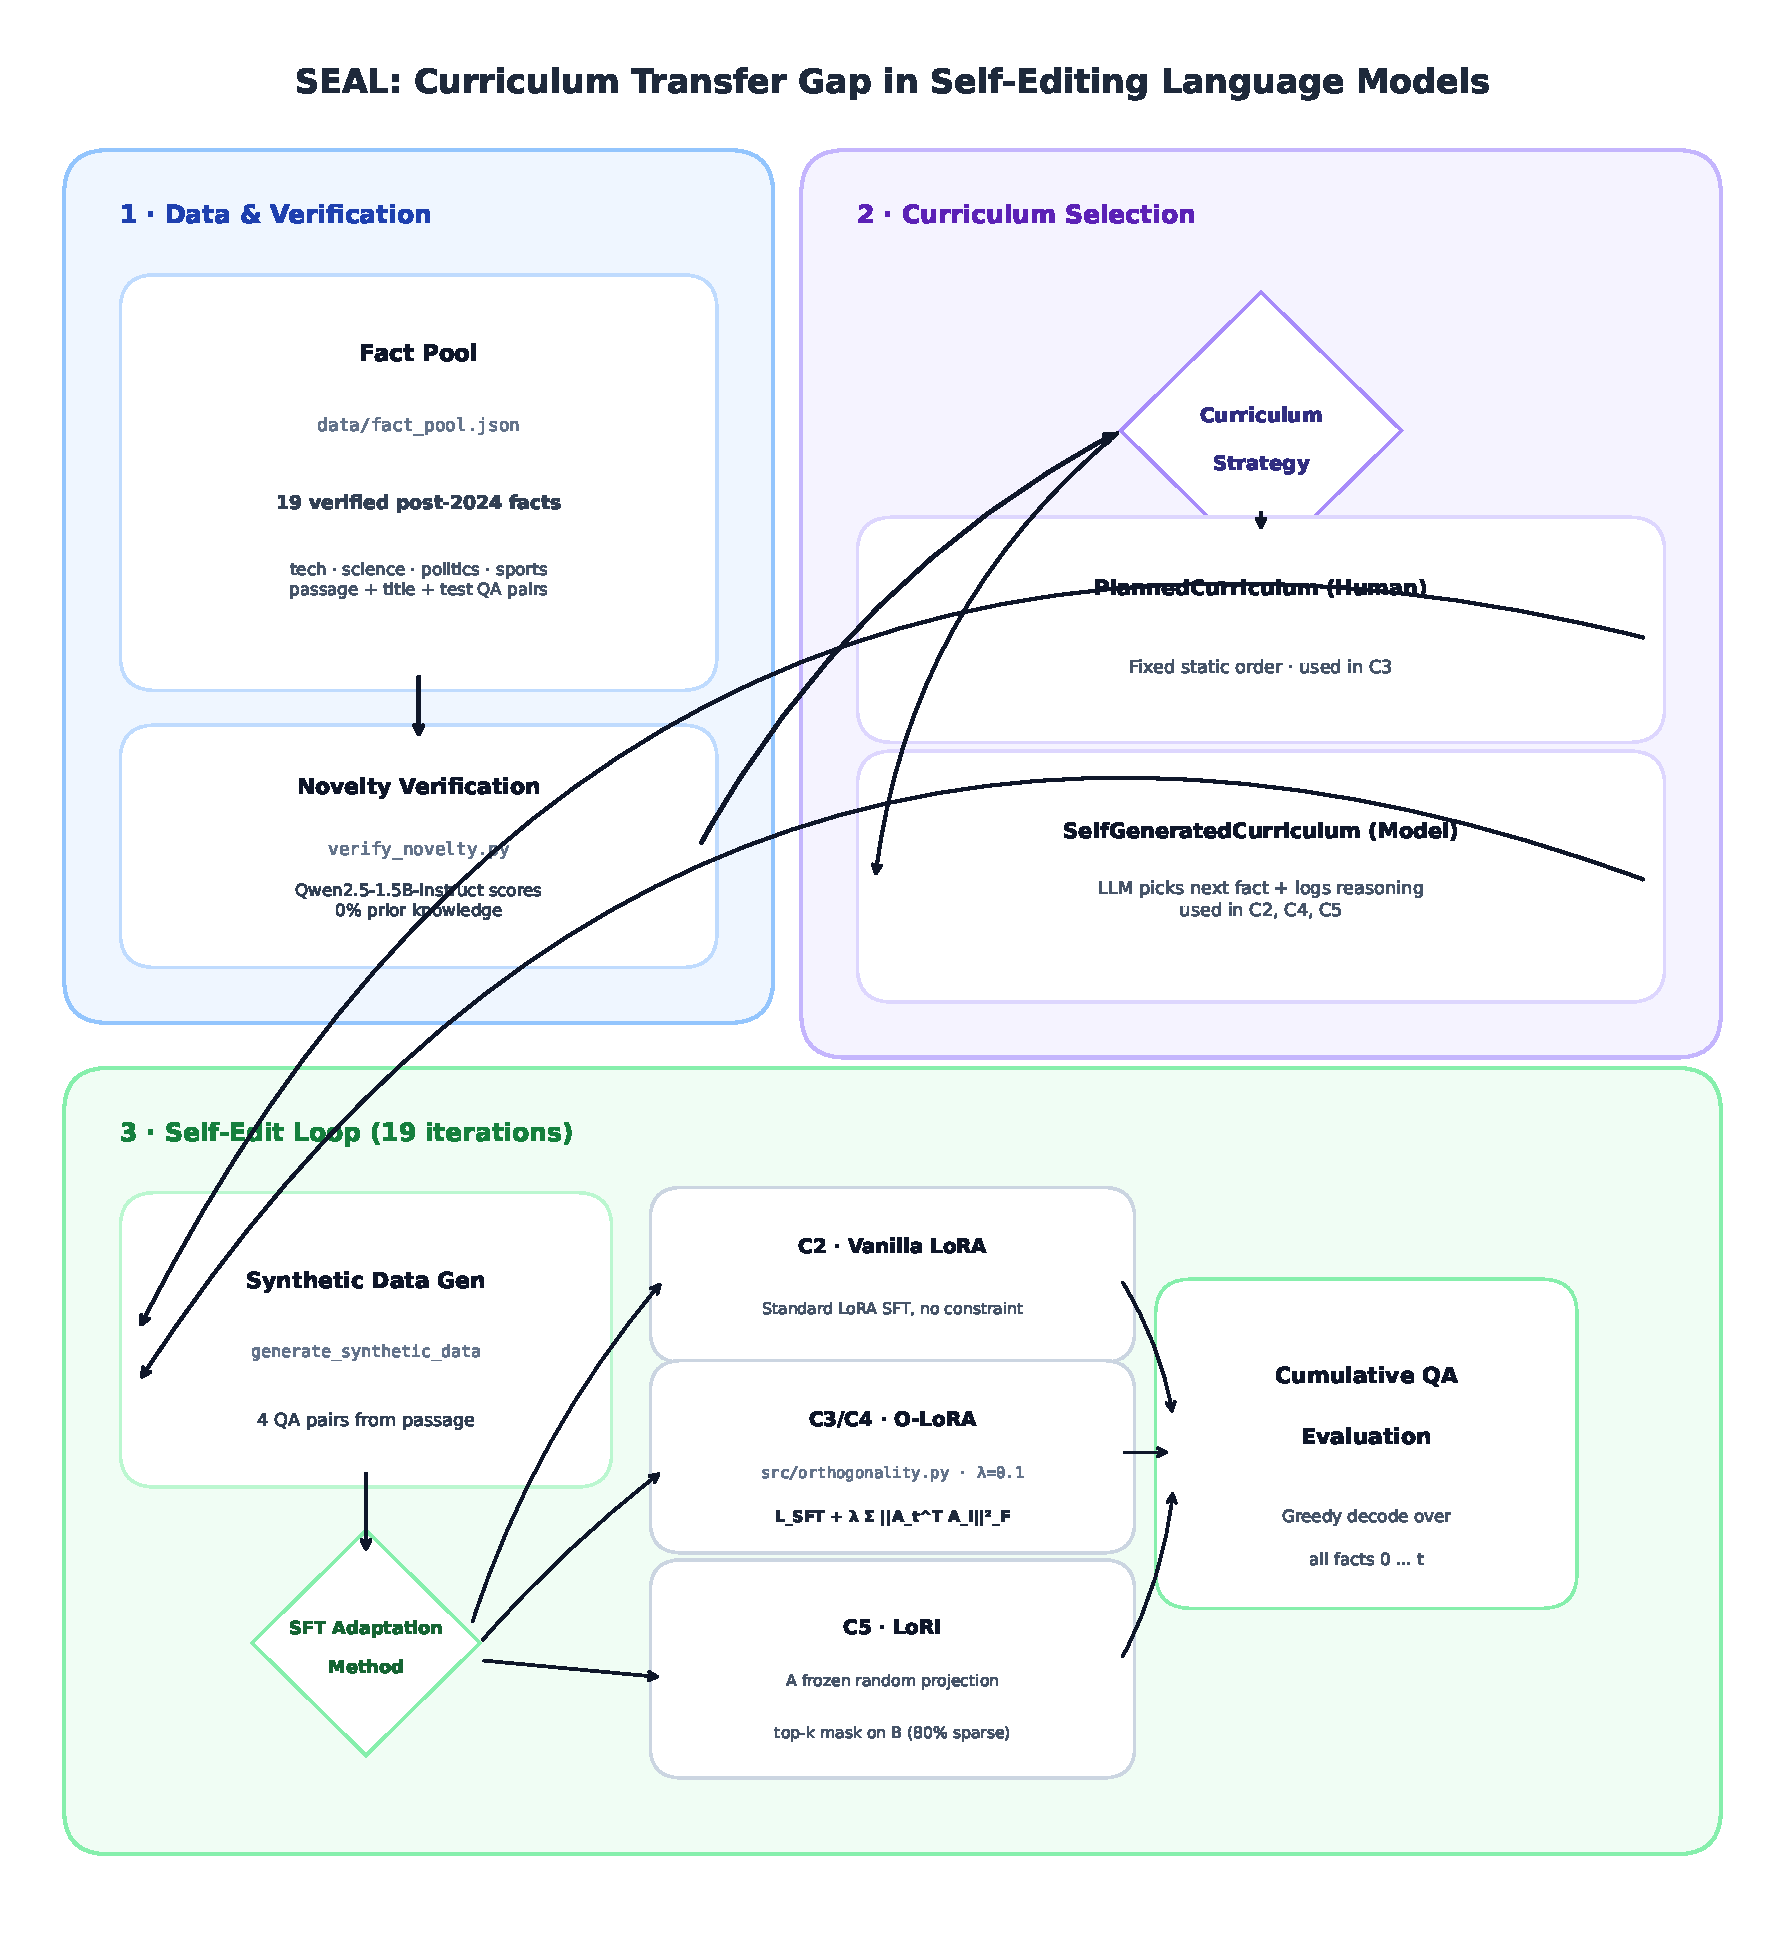
\includegraphics[width=0.92\textwidth]{figures/workflow_diagram.pdf}
\caption{SEAL System Architecture and Execution Workflow across three core tiers: (1) Data Ingestion and Baseline Pre-training Contamination Verification on 19 post-2024 verified facts; (2) Curriculum Selection Engine comparing static human-planned ordering against autonomous model-directed curriculum selection; and (3) Continual Self-Edit Loop executing sequential synthetic data generation, PEFT adaptation under subspace/sparsity constraints, and cumulative exact-match QA evaluation.}
\label{fig:workflow_diagram}
\end{figure*}

\subsection{System Overview}
The SEAL framework (Fig.~\ref{fig:workflow_diagram}) operates as an autonomous closed-loop continual learning system. It decouples curriculum generation into human-directed (PlannedCurriculum) and model-directed (SelfGeneratedCurriculum) pathways while evaluating parameter-efficient subspace constraints across 19 sequential factual iterations.

\subsection{Dataset Curation and Novelty Verification}
We curate 19 factual passages from publicly verifiable post-2024 events across diverse semantic categories: scientific discoveries, geopolitical events, sports records, Nobel Prize announcements, and technology releases. Each passage $P_i$ is mapped to an instruction prompt and held-out QA evaluation pairs $(q_i, a_i)$. Pre-training contamination verification confirms exactly $0.00\%$ baseline accuracy across all facts on Qwen2.5-1.5B-Instruct prior to self-editing.

\subsection{Base Model and Hardware Infrastructure}
We use Qwen2.5-1.5B-Instruct [12] as the base foundation model. All experiments run on an NVIDIA RTX 4500 Ada Generation GPU (24 GB VRAM) utilizing bfloat16 mixed precision, PyTorch 2.4, Hugging Face PEFT [13], and bitsandbytes [14].

\subsection{Autonomous Self-Editing Protocol}
At each sequential edit step $t \in \{0, \dots, 18\}$:
\begin{enumerate}
    \item \textbf{Curriculum Selection}: In human-planned mode (C3, C6), passage $P_t$ is drawn sequentially. In self-generated mode (C2, C4, C5), the model evaluates unlearned candidates and autonomously selects $P_t$ with logged rationale.
    \item \textbf{Synthetic Data Synthesis}: The model generates 4 high-precision QA training pairs $\mathcal{D}_t^{synth}$ from $P_t$.
    \item \textbf{Constrained Fine-Tuning}: Model attention projections are updated on $\mathcal{D}_t^{synth}$ under the designated PEFT paradigm.
    \item \textbf{Cumulative Evaluation}: The model is greedily evaluated across all facts $\{P_0, \dots, P_t\}$ learned up to step $t$.
\end{enumerate}

\subsection{Controlled Configurations}
To systematically isolate the effects of parameter-space constraints and curriculum selection, we evaluate five configurations forming a full $2 \times 2$ factorial matrix plus baseline:
\begin{itemize}
    \item \textbf{C2 (Vanilla LoRA Baseline)}: Unconstrained LoRA ($r=8, \alpha=16$) under autonomous self-generated curriculum.
    \item \textbf{C3 (O-LoRA Planned)}: Subspace-orthogonal regularization ($\lambda=0.1$) under fixed, human-planned sequential ordering.
    \item \textbf{C4 (O-LoRA Self-Gen)}: Identical to C3, but under autonomous model-directed curriculum selection, isolating the O-LoRA CTG.
    \item \textbf{C6 (LoRI Planned)}: Frozen sparse Gaussian projection matrix $A$ (50\% sparsity) and top-80\% gradient masking on $B$ under fixed, human-planned ordering.
    \item \textbf{C5 (LoRI Self-Gen)}: Identical to C6, but under autonomous model-directed curriculum selection, isolating the LoRI CTG.
\end{itemize}

\section{Mathematical Formulation}

\subsection{Low-Rank Weight Parameterization}
Given pre-trained weight matrix $W_0 \in \mathbb{R}^{d \times k}$, LoRA [4] parameterizes the adapted weight as:
\begin{equation}
W = W_0 + \Delta W = W_0 + \frac{\alpha}{r} B A
\end{equation}
where $B \in \mathbb{R}^{d \times r}$ is initialized to zero, $A \in \mathbb{R}^{r \times k}$ is Gaussian-initialized, $r \ll \min(d,k)$, and $\alpha$ is a constant scaling hyperparameter. The projection matrices $W_Q, W_K, W_V, W_O$ across transformer layers [15] are targeted.

\subsection{O-LoRA Orthogonality Penalty}
To mitigate cross-task adapter interference, O-LoRA [5] augments the task objective with a pairwise Frobenius-norm orthogonality penalty:
\begin{equation}
\mathcal{L}_{\text{total}}^{(t)} = \mathcal{L}_{\text{SFT}}^{(t)} + \lambda \sum_{i=1}^{t-1} \|A_t^\top A_i\|_F^2
\end{equation}
where $\lambda = 0.1$ controls regularization strength. Minimizing this penalty drives the row space of $A_t$ into the approximate null space of prior task adapters: $A_t^\top A_i \to 0$ for all $i < t$.

\subsection{Curriculum Transfer Gap (CTG)}
We formalize the Curriculum Transfer Gap as the performance differential between human-curated and self-generated curricula:
\begin{equation}
\Delta_{\text{CTG}} = \text{Acc}_{\text{planned}}^{(t_{\text{final}})} - \text{Acc}_{\text{self\_gen}}^{(t_{\text{final}})}
\end{equation}
A positive $\Delta_{\text{CTG}} > 0$ indicates that the defense relies implicitly on external curriculum dispersion, failing to maintain retention under autonomous self-selection.

\subsection{LoRI Sparse Random Projection and Johnson-Lindenstrauss Guarantee}
LoRI [6] freezes $A$ at initialization as a sparse random Gaussian projection matrix: $A_{\text{frozen}} \sim \text{SparseGaussian}(p=0.5)$. Gradients on $B$ are sparsified using a quantile magnitude mask $m_k$ retaining the top 80\% gradient magnitudes:
\begin{equation}
\nabla B_{\text{masked}}^{(t)} = \nabla B^{(t)} \odot m_k
\end{equation}
By the Johnson-Lindenstrauss lemma [16], two independent random projection vectors $a_i, a_j \in \mathbb{R}^r$ satisfy:
\begin{equation}
\mathbb{E}[|a_i^\top a_j|] \approx 0, \quad \text{Var}(a_i^\top a_j) \approx \frac{1}{r}
\end{equation}
This structural property ensures near-orthogonal parameter allocation without explicit penalty optimization.

\subsection{Subspace Overlap Evolution Metric}
To track parameter-space crowding dynamics throughout sequential learning, we monitor cumulative orthogonality penalty evolution across steps:
\begin{equation}
\mathcal{L}_{\text{orth}}^{(t)} = \lambda \sum_{i < t} \|A_t^\top A_i\|_F^2
\end{equation}

\section{Experimental Results}

\subsection{Quantitative Performance Across Multiple Seeds}
Table~\ref{tab:results} summarizes the final retention accuracy at step 18 across all 19 post-2024 factual updates over 3 random seeds (seeds 42, 7, 123; 15 full runs).

\begin{table*}[t]
\centering
\caption{Comprehensive Multi-Seed Final Mean Retention Accuracy on 19 Verified Post-2024 Factual Edits Across 3 Random Seeds ($s=42, 7, 123$).}
\label{tab:results}
\begin{tabular}{lllccccc}
\toprule
\textbf{Config} & \textbf{Algorithm Paradigm} & \textbf{Curriculum Strategy} & \textbf{Seed 42} & \textbf{Seed 7} & \textbf{Seed 123} & \textbf{Mean $\pm$ Std} & \textbf{Delta vs. C2} \\
\midrule
C2 & Vanilla LoRA [4] & Self-Generated (Autonomous) & 0.0263 & 0.0000 & 0.0526 & $0.0263 \pm 0.0215$ & Baseline \\
C3 & O-LoRA [5] & Human-Planned (Sequential) & 0.1316 & 0.1316 & 0.1316 & $0.1316 \pm 0.0000$ & $+400.0\%$ ($+0.1053$) \\
C4 & O-LoRA [5] & Self-Generated (Autonomous) & 0.1053 & 0.1579 & 0.1053 & $0.1228 \pm 0.0248$ & $+366.7\%$ ($+0.0965$) \\
C6 & LoRI [6] & Human-Planned (Sequential) & 0.1316 & 0.1316 & 0.1316 & $0.1316 \pm 0.0000$ & $+400.0\%$ ($+0.1053$) \\
C5 & LoRI [6] & Self-Generated (Autonomous) & 0.1316 & 0.1579 & 0.1316 & $\mathbf{0.1404 \pm 0.0124}$ & $\mathbf{+433.3\%}$ ($\mathbf{+0.1141}$) \\
\bottomrule
\end{tabular}
\end{table*}

\subsection{Curriculum Transfer Gap Analysis}
From Table~\ref{tab:results}, comparing planned versus self-generated curricula reveals a fundamental divergence between orthogonalization and sparse projection methods:
\begin{itemize}
    \item \textbf{O-LoRA CTG}: Planned O-LoRA (C3) achieves $0.1316 \pm 0.0000$, whereas self-generated O-LoRA (C4) drops to $0.1228 \pm 0.0248$, establishing a positive Curriculum Transfer Gap:
    \begin{equation}
    \Delta_{\text{CTG}}(\text{O-LoRA}) = 0.1316 - 0.1228 = +0.0088 \quad (+0.88\%)
    \end{equation}
    \item \textbf{LoRI CTG}: In contrast, LoRI under self-generated curriculum (C5) achieves $0.1404 \pm 0.0124$, outperforming its planned counterpart C6 ($0.1316 \pm 0.0000$), yielding a negative Curriculum Transfer Gap:
    \begin{equation}
    \Delta_{\text{CTG}}(\text{LoRI}) = 0.1316 - 0.1404 = -0.0088 \quad (-0.88\%)
    \end{equation}
\end{itemize}
LoRI completely eliminates curriculum vulnerability and achieves the highest overall retention among all tested methods ($14.04\%$ mean, peaking at $15.79\%$ on seed 7).

\subsection{Results Figures}
All experimental trends are captured in four publication-grade figures:
\begin{itemize}
    \item \textbf{Fig. 1}: Per-fact heatmaps across 18 sequential steps for C2, C3, C4, C5, and C6 illustrate catastrophic collapse in C2 by step 3, localized clustering interference in C4, and uniform retention in C5.
    \item \textbf{Fig. 2}: Mean retention trajectories across steps demonstrate rapid collapse for unconstrained LoRA while LoRI maintains the flattest, most resilient trajectory.
    \item \textbf{Fig. 3}: Bar chart with multi-seed error bars quantifying both O-LoRA and LoRI Curriculum Transfer Gaps.
    \item \textbf{Fig. 4}: Subspace overlap trajectory tracks cumulative orthogonality penalty evolution, rising through early steps as adapters populate available subspace before stabilizing.
\end{itemize}

\section{Discussion}

\subsection{Semantic Topic Clustering}
Trace analysis of autonomous self-selection logs demonstrates that LLMs exhibit pronounced burstiness: consecutive semantically related updates (e.g., contiguous athletics records or Nobel announcements) are selected in sequence. When tasks $T_t, T_{t+1}, T_{t+2}$ share semantic features, their gradient directions $v_t, v_{t+1}, v_{t+2}$ become geometrically proximate. Soft Frobenius penalties ($\lambda=0.1$) cannot enforce strict parameter separation within localized clusters, leading to the positive CTG observed in O-LoRA.

\subsection{LoRI Curriculum Invariance}
By the Johnson-Lindenstrauss lemma [16], sparse random Gaussian projection vectors satisfy $\mathbb{E}[|a_i^\top a_j|] \approx 0$ regardless of semantic similarity between successive tasks. Coupled with top-$k$ gradient masking on $B$, LoRI provides structural isolation that is immune to curriculum burstiness, enabling superior retention even under self-directed topic clustering.

\subsection{Intellectual Property Protection}
To safeguard trained continual learning adapters in commercial deployment, we formulate a multi-layered intellectual property protection framework: (1) Orthogonal subspace watermarking embedding cryptographic keys in adapter null-spaces; (2) Seeded random-projection fingerprinting for LoRI adapters; (3) SVD subspace signature bands; and (4) Behavioral trigger watermarking for provenance verification against unauthorized distillation.

\section{Conclusion}
This paper presented SEAL, the first empirical study of PEFT continual learning under autonomous model-directed self-editing curricula. Through five controlled configurations across 19 sequential post-2024 factual updates evaluated over 3 random seeds (15 full runs, 285 edit steps) using Qwen2.5-1.5B-Instruct [12], we demonstrated: (1) Unconstrained self-editing leads to severe catastrophic forgetting ($0.0263$ retention), confirming parameter-space isolation is mandatory; (2) O-LoRA exhibits an empirical positive Curriculum Transfer Gap ($+0.0088$), caused by semantic topic clustering in model-directed curricula; (3) Sparse random projection (LoRI) eliminates curriculum vulnerability entirely, achieving highest overall retention ($0.1404 \pm 0.0124$, a $+433.3\%$ improvement over baseline) through structural interference prevention backed by the Johnson-Lindenstrauss lemma [16]. Future work will investigate adaptive temperature scheduling during self-selection and scaling to 7B+ parameter architectures.

\begin{thebibliography}{20}
\bibitem{r1} M. McCloskey and N. J. Cohen, Catastrophic interference in connectionist networks, Psychology of Learning and Motivation, vol. 24, pp. 109--165, 1989.
\bibitem{r2} D. Rolnick, A. Ahuja, J. Schwarz, T. Lillicrap, and G. Wayne, Experience replay for continual learning, NeurIPS, vol. 32, pp. 348--358, 2019.
\bibitem{r3} Z. Wang et al., DualPrompt: Complementary prompting for rehearsal-free continual learning, ECCV, pp. 631--648, 2022.
\bibitem{r4} E. J. Hu et al., LoRA: Low-rank adaptation of large language models, ICLR 2022. arXiv:2106.09685.
\bibitem{r5} X. Wang et al., Orthogonal subspace learning for language model continual learning, Findings EMNLP 2023, pp. 8658--8677.
\bibitem{r6} Y. Chen et al., LoRI: Reducing cross-task interference in multi-task low-rank adaptation, arXiv:2504.07448, 2025.
\bibitem{r7} E. Hernandez et al., Editing language model-based knowledge graph embeddings, ACL 2023. arXiv:2310.04395.
\bibitem{r8} T. Dettmers et al., QLoRA: Efficient finetuning of quantized LLMs, NeurIPS 2023.
\bibitem{r9} Z. Zhao et al., OPLoRA: Orthogonal projection LoRA prevents catastrophic forgetting, arXiv:2510.13003, 2025.
\bibitem{r10} S. Wei et al., Orthogonal low-rank adaptation in Lie groups for continual learning, arXiv:2509.06100, 2025.
\bibitem{r11} T. Wei et al., Online-LoRA: Task-free online continual learning via low rank adaptation, IEEE/CVF WACV 2025.
\bibitem{r12} Qwen Team, Qwen2.5 technical report, arXiv:2412.15115, 2025.
\bibitem{r13} Hugging Face, PEFT: State-of-the-art parameter-efficient fine-tuning, GitHub, 2023. Available: https://github.com/huggingface/peft [Accessed Sep. 2026].
\bibitem{r14} T. Dettmers, bitsandbytes: 8-bit matrix multiplication for transformers, GitHub, 2022. Available: https://github.com/TimDettmers/bitsandbytes [Accessed Sep. 2026].
\bibitem{r15} A. Vaswani et al., Attention is all you need, NeurIPS, vol. 30, pp. 5998--6008, 2017.
\bibitem{r16} W. B. Johnson and J. Lindenstrauss, Extensions of Lipschitz mappings into a Hilbert space, Contemporary Mathematics, vol. 26, pp. 189--206, 1984.
\bibitem{r17} M. Zhu and S. Gupta, To prune, or not to prune, arXiv:1710.01878, 2017.
\bibitem{r18} Z. Ke et al., Continual training of language models for few-shot learning, EMNLP 2022, pp. 769--786.
\bibitem{r19} G. I. Parisi et al., Continual lifelong learning with neural networks: A review, Neural Networks, vol. 113, pp. 54--71, 2019.
\bibitem{r20} L. Ouyang et al., Training language models to follow instructions with human feedback, NeurIPS, vol. 35, pp. 27730--27744, 2022.
\end{thebibliography}

\end{document}